\documentclass[margin=0.1in]{standalone}
\usepackage{tikz}
\begin{document}

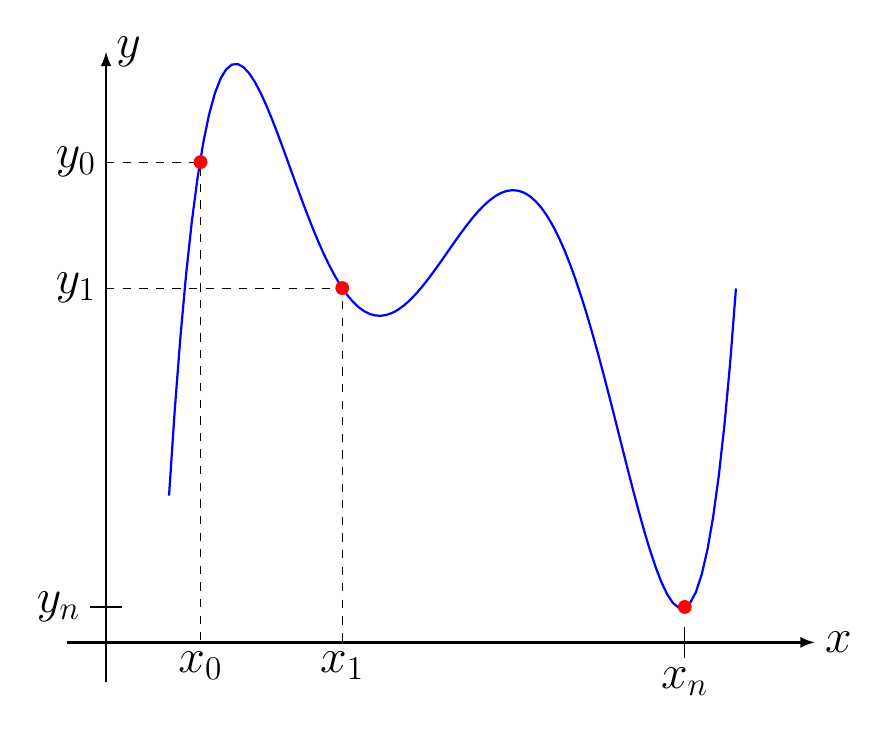
\begin{tikzpicture}[>=latex]
	\draw [->,thick] (-5.5,-2.5) -- (4,-2.5) node [right] {\LARGE  \(x\)};
	\draw [->,thick] (-5,-3) --++ (0,8) node [right] {\LARGE  \(y\)};
	\draw [thick , blue, domain=-4.2:3, samples = 100] plot(\x , {(\x+4) *(\x+2) *(\x+1) *(\x-1) *(\x-3)/20 +2});
	\draw [dashed] (-5,3.6) node [left] {\LARGE\(y_0\)} -- (-3.8,3.6) -- (-3.8,-2.5) node [below] {\LARGE \(x_0\)};
	\draw [dashed] (-5,2) node [left] {\LARGE \(y_1\)} -- (-2,2) -- (-2,-2.5) node [below] {\LARGE \(x_1\)};
	\draw (-4.8,-2.05) --++ (-0.4,0) node [left] {\LARGE \(y_n\)};
	\draw (2.35,-2.3) --++ (0,-0.4) node [below] {\LARGE \(x_n\)};
	\fill [red] (2.35,-2.05) circle (2.5pt);
	\fill [red] (-3.8,3.6) circle (2.5pt);
	\fill [red] (-2,2) circle (2.5pt);
\end{tikzpicture}

\end{document}
